\documentclass[a4,10pt]{article} \usepackage[pdftex]{graphicx}
\usepackage{setspace}
\usepackage{hyperref}
\hypersetup{
    colorlinks,%
    citecolor=black,%
    filecolor=black,%
    linkcolor=black,%
    urlcolor=blue
}


\pdfinfo{
   /Author (Ron Keizer, Coen van Hasselt, Pirana Software & Consulting BV)
   /Title  (Pirana Quick Guide)
}

%\usepackage{lineno}
\usepackage{color}
\definecolor{PiranaOrange}{rgb}{0.9,0.4,0.1}
\definecolor{Blue}{rgb}{0.0,0.0,0.7}
\definecolor{Red}{rgb}{0.7,0.0,0.0}
\definecolor{Grey}{rgb}{0.2,0.2,0.2}
\definecolor{grey2}{rgb}{.92, .92, .92}

\bibliographystyle{unsrt}%Choose a bibliograhpic style}
%\usepackage{utopia} %\usepackage{charter} %\usepackage{palatino}
%\usepackage{bookman} %\usepackage{newcent} %\usepackage{times}
%\usepackage[options]{natbib} \sloppy
\renewcommand{\familydefault}{\sfdefault} 
\renewcommand{\emph}[1]{\textbf{\textcolor{Grey}{#1}}} 
\oddsidemargin 1cm
\textwidth 14cm
\textheight 20cm

\begin{document}

{\centering
  \vspace{-100pt}
  \textbf{
    \textcolor{PiranaOrange}{\Large Pirana}
  }\\
  \vspace{5pt} \scriptsize \textcolor{Grey}{The flexible modeling
    environment for NONMEM} \\ \normalsize
  \vspace{12pt}
  \hspace{5pt}
\includegraphics[scale=0.14]{images/pirana_logo.jpg}\\
  \vspace{18pt}
  {\large
    \emph{Quick Guide: Making VPC's with PsN and Xpose}  \vspace{10pt} \\
    Version 1.1
  }

}
\vspace{25pt}


\begin{center}
   {\colorbox{grey2}{
         \begin{minipage}[t]{0.9\textwidth}
\subsubsection*{Scope}
This Pirana Quick Guide explains how to use Pirana to generate VPC
data using PsN, and how to subsequently use that data to create VPC plots
with Xpose using different plotting options. 
          \end{minipage}
      }
   }
\end{center}

\subsubsection*{Generating data for the VPC}
\begin{itemize}
\item Select the model for which a VPC should be created, and select
  the option VPC via the menu below your right-mouse button (PsN $
  \rightarrow$ Model evaluation $ \rightarrow$ vpc) (Figure \ref{fig:Fig1}).
\end{itemize}

\begin{figure}[h] \centering
    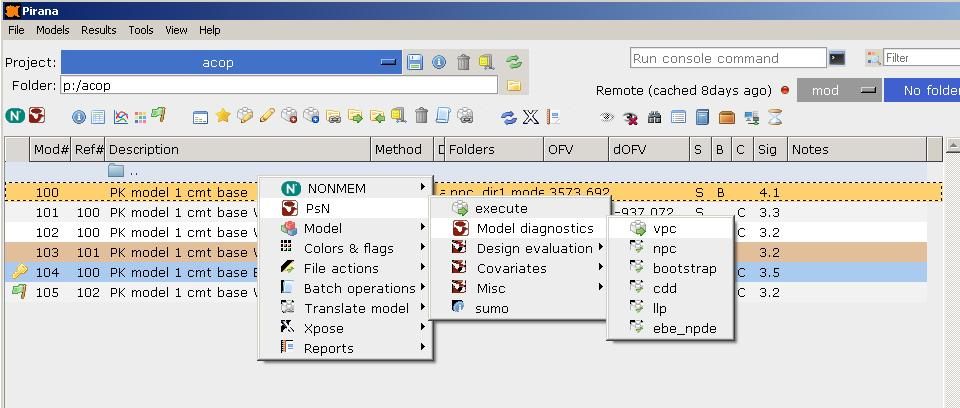
\includegraphics[scale=.4]{images/vpc_1.jpg}
    \caption{Selecting a run and executing the PsN/VPC Toolkit run window
     \label{fig:Fig1}}
\end{figure}

\begin{itemize}
\item In the resulting PsN settings window, the command for running
  creating the vpc can be specified (Figure \ref{fig:Fig2}). The vpc command takes
  many arguments which alters the way the vpc is calculated, e.g. you
  can specify stratifications, binning, dependent variable etc.
\item Arguments may be added in the text box at the lower part of the
  PsN run window (orange square). Make sure to separate the arguments
  by a space, and start each argument with a `-'.
\item A full overview of possible arguments and their use may be
  viewed in the upper part of the PsN run window. By clicking on
  `Help', additional help on these arguments is available (small blue square).
\item When all arguments for the VPC dataset have been defined
  correctly, the PsN/vpc run may be executed (green square).
\end{itemize}

\begin{figure}[h] \centering
    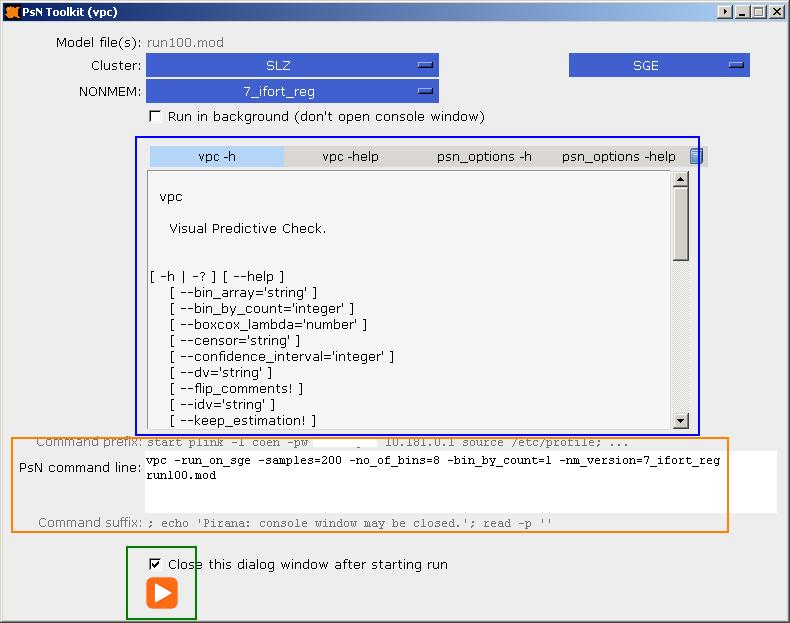
\includegraphics[scale=.4]{images/vpc_2.jpg}
    \caption{PsN/vpc Toolkit run window
     \label{fig:Fig2}}
\end{figure}

\begin{itemize}
\item If the VPC run is not executed in the background, a run window
  will appear similiar to Figure Figure \ref{fig:Fig3}. Make sure to check if no errors
  are reported in this step. If the vpc finishes correctly, it will
  report something like `Done reading and formatting data, finishing run.'
\end{itemize}

\begin{figure}[h] \centering
    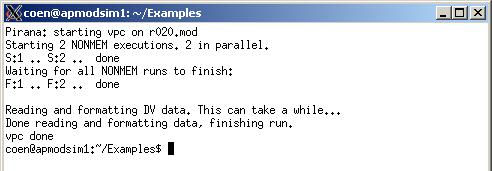
\includegraphics[scale=.5]{images/vpc_3.jpg}
    \caption{Output after execution of VPC run using PsN
    \label{fig:Fig3}}
\end{figure}

\subsubsection*{Plotting the VPC data}

\begin{itemize}
\item If the VPC was run succesfull, a new folder will be created
  which is named npc\_dirX, at least if you did not specify another
  folder name manually (Figure \ref{fig:Fig3}, blue square).
\item If you don't see the folder yet in Pirana, press the folder
  refresh button (round green/white button). Also make sure that the folder filter is set to
  \emph{PsN folders} or \emph{All folders} (Figure \ref{fig:Fig3}, orange square).
\item Note that if you run the vpc command multiple times, multiple
  \emph{npc\_dir} folders will be created. It is therefore advisable
  to use the `-dir' option in PsN to specify a specific folder each
  time you run a vpc.
\end{itemize}

\begin{figure}[h] \centering
    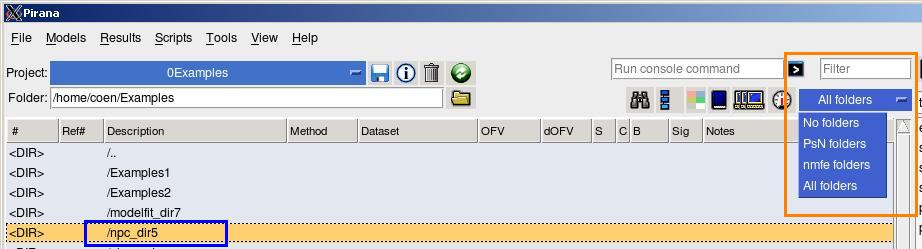
\includegraphics[scale=.35]{images/vpc_4.jpg}
    \caption{VPC run folder created after execution of VPC run
    \label{fig:Fig4}}
\end{figure}

\begin{itemize}
\item Select the model for which the VPC was executed. (Figure \ref{fig:Fig5}).
\item Select Xpose $\rightarrow$ Run Xpose commands. This will open up
  the Pirana Xpose interface.
\end{itemize}

\begin{figure}[h] \centering
    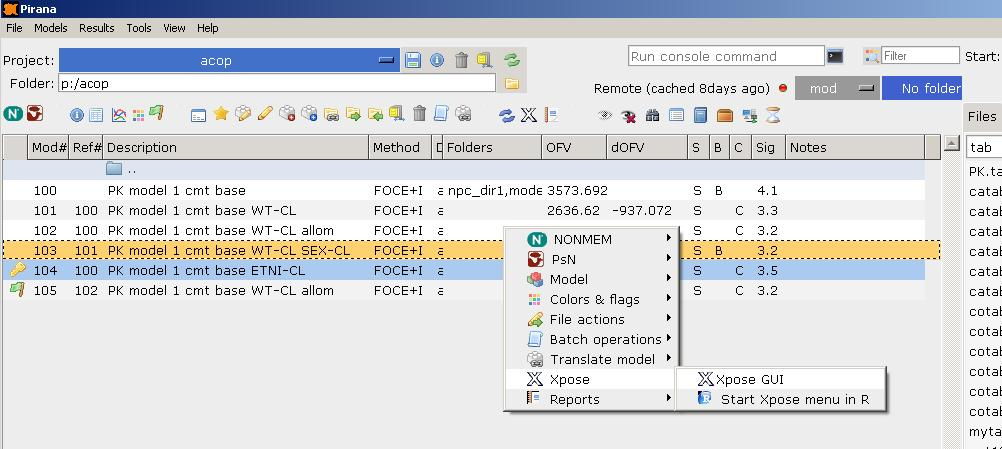
\includegraphics[scale=.4]{images/vpc_5.jpg}
    \caption{Starting the 'Run Xpose commands' window on selected run.
    \label{fig:Fig5}}
\end{figure}

\begin{itemize}
\item Enter or select xpose.VPC in the command text field (Figure \ref{fig:Fig6},
  blue square). If any other commands are present in the list, remove these.
\item Next, arguments for the Xpose.VPC may be added (Figure \ref{fig:Fig6}, orange
  square).  The xpose.VPC help files may be accessed using the help
  button.
\item Several options are available for the output format. The easiest
  option is to automatically generate the graph and save as PDF
  (default) or PNG file (Figure \ref{fig:Fig6}, red square).
\item Alternative output formats are to generate the R-code only and
  open it in your R interface, or to to generate Sweave code for LaTeX
  documents.
\item If all settings have been configured, the VPC may be generated
  by pressing the execute button (Figure \ref{fig:Fig6}, green square).
\item If output was directed to a PDF or PNG file, this file will be 
  automatically opened by the PDF viewer you specified in Pirana's
  settings. (Figure \ref{fig:Fig7}). If you choose to generate R or LaTeX code,
  Pirana will open the R GUI or your code editor, and you will have to
  run the generated code manually.
\end{itemize}

\subsubsection*{Tweaking the VPC plot}
These VPCs may be further optimized by adjusting the many Xpose
arguments. Please check out the xpose VPC help files (which may be
accessed from the Run Xpose command window, or go the the Xpose
website for more information).

\begin{figure}[h] \centering
    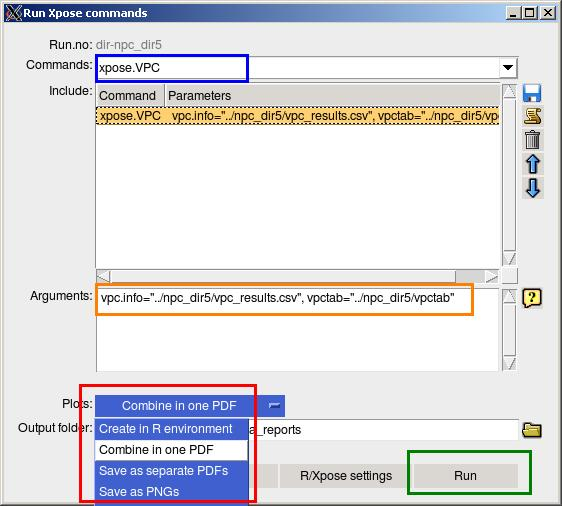
\includegraphics[scale=.4]{images/vpc_6.jpg}
    \caption{The 'Run Xpose commands' window to generate the VPC graph
      \label{fig:Fig6}}
\end{figure}

\begin{figure}[h] \centering
    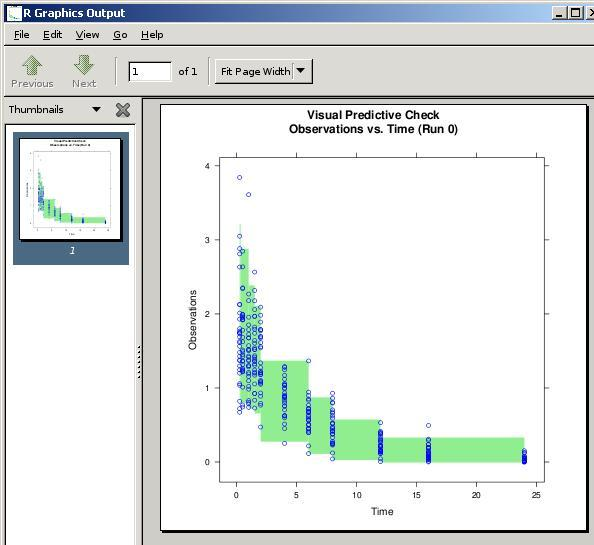
\includegraphics[scale=.4]{images/vpc_7.jpg}
    \caption{VPC obtained through PsN and Xpose
      \label{fig:Fig7}}
\end{figure}


\end{document}
